\PassOptionsToPackage{implicit=true}{hyperref}
\documentclass[10pt, aspectratio=169, compress, protectframetitle, handout]{beamer}
\usepackage[utf8]{inputenc}
\usepackage[english]{babel}
\usepackage{appendixnumberbeamer}
% handout to deactivate \uncover
% usetitleprogressbar might be needed
%\usepackage{beamerprosper}
\usepackage{comment}
% Load BEFORE the theme
\usepackage[normalem]{ulem}
\usepackage[T1]{fontenc}

\usetheme[progressbar=frametitle,block=fill,numbering=fraction]{metropolis}
\setbeamertemplate{blocks}[rounded][shadow=true]

% Change Colors/Width of Progress Bars 
\makeatletter
%\setlength{\metropolis@titleseparator@linewidth}{1pt}
\setlength{\metropolis@progressonsectionpage@linewidth}{0.8pt}
\setlength{\metropolis@progressinheadfoot@linewidth}{1pt}
\makeatother

%\setbeamertemplate{note page}[plain]
%\setsansfont[
%     Extension      = .otf,
%     UprightFont    = *-Light,
%     ItalicFont     = *-LightItalic,
%     BoldFont       = *-Regular,
%     BoldItalicFont = *-RegularItalic
% ]{FiraSans}
%\setmonofont[
%     Extension   = .otf,
%     UprightFont = *-Regular,
%     BoldFont    = *-Medium
%]{FiraMono}


\newcommand{\putbg}{\usebackgroundtemplate{
\includegraphics[width=\paperwidth,height=\paperheight]{background-vector_169}}}
\newcommand{\putbgdark}{\usebackgroundtemplate{
\includegraphics[width=\paperwidth,height=\paperheight]{background-vector-dark_169}}}


\usepackage[export]{adjustbox}
\usepackage[]{enumitem}
\usepackage{datetime}
\usepackage{textpos}
\usepackage{xcolor}
\usepackage{marvosym} % Smile
\usepackage{fontawesome5} % Icons
\usepackage{wrapfig} % To wrap figures wih text
\usepackage{cleveref} % To fix autoref links not working
% Fixes bad positioning of hats
\usefonttheme{professionalfonts}%[onlymath]{serif}
\PassOptionsToPackage{hyphens}{url}\usepackage{hyperref} % to break the links
\hypersetup{
    colorlinks=true,
    linkcolor=,      % color of internal links
    urlcolor=blue,   % color of external links
    citecolor=blue,  % color of links to bibliography
}


%%% Bibliografia
\usepackage[autostyle]{csquotes}
\usepackage[backend=biber]{biblatex}

% https://tex.stackexchange.com/questions/68080/beamer-bibliography-icon
\setbeamertemplate{bibliography item}{%
  \ifboolexpr{ test {\ifentrytype{book}} or test {\ifentrytype{mvbook}}
    or test {\ifentrytype{collection}} or test {\ifentrytype{mvcollection}}
    or test {\ifentrytype{reference}} or test {\ifentrytype{mvreference}} }
    {\setbeamertemplate{bibliography item}[book]}
    {\ifentrytype{online}
       {\setbeamertemplate{bibliography item}[online]}
       {\setbeamertemplate{bibliography item}[article]}}%
  \usebeamertemplate{bibliography item}}

\defbibenvironment{bibliography}
  {\list{}
     {\settowidth{\labelwidth}{\usebeamertemplate{bibliography item}}%
      \setlength{\leftmargin}{\labelwidth}%
      \setlength{\labelsep}{\biblabelsep}%
      \addtolength{\leftmargin}{\labelsep}%
      \setlength{\itemsep}{\bibitemsep}%
      \setlength{\parsep}{\bibparsep}}}
  {\endlist}
  {\item}

\addbibresource{biblio.bib}


%%% Metadati
\graphicspath{{figures/PNG/}{figures/PDF/}{figures/}}
\newdateformat{monthyear}{\monthname[\THEMONTH] \THEYEAR}
\title{\vspace*{1.5cm}How to crack (kind of) the videogame ``Breakout''}
\subtitle{A project for the \emph{Reinforcement Learning} course}
\author{Angela Carraro}
\date{}
\institute{\scshape DSSC - UniTS
\vfill

\includegraphics[valign=c, height=0.7cm]{logo_dssc_alt}
\hspace*{0.5cm}

\includegraphics[valign=c, height=0.75cm]{Logo_units_blu}
}

\addtobeamertemplate{frametitle}{}{%
\begin{textblock*}{100mm}(0.90\textwidth,-0.94cm)

\includegraphics[valign=c, height=0.4cm]{logo_dssc_alt_white}

\includegraphics[valign=c, height=0.45cm]{Logo_units_white}
\end{textblock*}}

\begin{document}

{\putbg\maketitle}


%\begin{frame}{Contents}
%	\tableofcontents
%\end{frame}


\begin{frame}{Aim of the project}

    Teach a computer agent to play the Atari 2600 game Breakout via the Reinforcement Learning technique of Double (Deep) Q-Learning.
    
    We will use images of the screen game to make our agent learn a policy that can allow it to score a sufficient number of points in the game (how many depends on the computing power and the time at your disposal).
    
    \begin{columns}[onlytextwidth]
        \begin{column}{.4\textwidth}
            \begin{description}[align=right,labelindent=4cm] % 3cm
                \item[\alert{Language}] Python
                \item[\alert{Game Environment}] Gym
                \item[\alert{ML framework}] PyTorch
                \item[\alert{Cluster}] Ulysses
            \end{description}
        \end{column}
        \begin{column}{.6\textwidth}
            \begin{figure}
                \centering
                
\includegraphics[width=3.5cm]{figures/Atari_trimmed.png}
            \end{figure}
        \end{column}
    \end{columns}
    
\end{frame}


{\putbg
\section{The Game}
}


\begin{frame}{Breakout}
    
    The game begins with $6$ rows of different colors of $18$ bricks each. After firing the ball (red button on the Atari console), the player must knock down as many bricks as possible by using the walls and/or the paddle below to bounce the ball against the bricks and eliminate them.
    
    \begin{columns}[onlytextwidth]
        \begin{column}{.7\textwidth}
            If the player's paddle misses the ball's rebound, they will lose a life, the ball will disappear from the screen and they would have to press the red controller button to serve another ball.
            \smallskip
            
            %After observing DeepMind's \href{https://www.youtube.com/watch?v=TmPfTpjtdgg}{video}, I've learnt that:
            The color of a brick determines the points you score when you hit it with your ball. In the official Atari 2600 game \href{https://atariage.com/manual_html_page.php?SoftwareID=889}{\underline{rules}}, there is stated that:
            \begin{itemize}
                \item[$\bullet$] {\color[RGB]{70,73,205}Blue} and {\color[RGB]{72,150,76}green} bricks earn $1$ point each.
                \item[$\bullet$] {\color[RGB]{162,162,42}Yellow} and {\color[RGB]{187,123,60}light orange} bricks earn $4$ points each.
                \item[$\bullet$] {\color[RGB]{215,113,64}Dark orange} and {\color[RGB]{218,82,77}red} bricks score $7$ points each.
            \end{itemize}
        \end{column}
        \begin{column}{.3\textwidth}
            \begin{figure}
                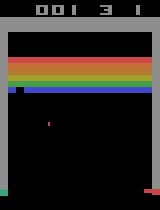
\includegraphics[width=3.8cm]{figures/poster}
                %\caption{The game.}
            \end{figure}
        \end{column}
    \end{columns}
    
\end{frame}


\begin{frame}{Breakout}

        \begin{columns}[onlytextwidth]
        \begin{column}{.4\textwidth}
            \begin{figure}
                \centering
                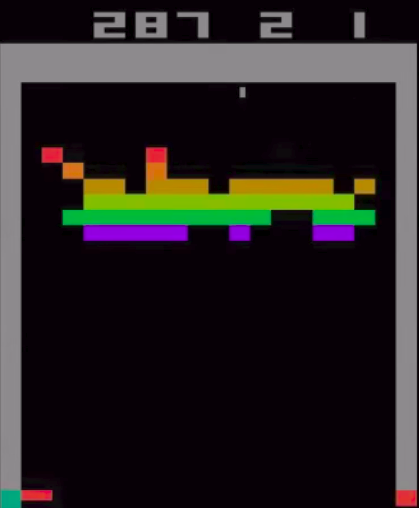
\includegraphics[width=3.8cm]{figures/poster2}
                \caption{Optimal strategy to solve this game: make a tunnel around the side, and then allow the ball to hit blocks by bouncing behind the wall.}
            \end{figure}
        \end{column}
        \begin{column}{.55\textwidth}
        
            The score is displayed at the top left of the screen (maximum for clearing one screen is $448$ points), the number of lives remaining is shown in the middle (starting with $5$ lives), and the ``1'' on the top right indicates this is a 1-player game.
            \medskip
            
            The paddle shrinks after the ball has broken through the red row and hit the upper wall.
            \medskip
            
            The ball speed increases at specific intervals: after four hits, after twelve hits, and after making contact with the orange and red rows.
        \end{column}
    \end{columns}
    
\end{frame}


\begin{frame}{The specifications}

    We will use the environment of OpenAI's library \href{https://gym.openai.com/}{Gym} $\big[$doc (scarce) available \href{https://gym.openai.com/envs/Breakout-v0/}{here}$\big]$.
    
    In the environment a frame-skipping technique is implemented. More precisely, the agent sees and selects actions on every $k$-th frame, instead of every frame, and its last action is repeated on skipped frames.
    
    There are different options you can specify when setting the environment. If you look at the \texttt{atari\_env} \href{https://github.com/openai/gym/blob/master/gym/envs/__init__.py\#L603}{source code} (explained well in this \href{https://github.com/openai/gym/issues/1280}{link}), you can add one of these options after the game name \texttt{Breakout}:
    \begin{itemize}
        \item[\alert{$\bullet$}] \texttt{-v0} or \texttt{-v4}: \texttt{-v0} has \texttt{repeat\_action\_probability} of $0.25$ (meaning $25\%$ of the time the previous action will be used instead of the new action), while \texttt{-v4} has $0$ (always follow your issued action).
    
        \item[\alert{$\bullet$}] \texttt{Deterministic}: it keeps a fixed frameskip of $4$, while for the env without \textsc{Deterministic} the frameskip $k$ is uniformly sampled from $\{2, 3, 4\}$ (code \href{https://github.com/openai/gym/blob/master/gym/envs/atari/atari_env.py\#L24}{here}).
        
        \item[\alert{$\bullet$}] \texttt{NoFrameskip}: a fixed frameskip of $1$, which means we get every frame, so no frameskip.
        
    \end{itemize}
    
    %So \textsc{NoFrameskip-v4} will have no frame skip and no action repeat stochasticity.
    
    %You can have a random number of frames being skipped each time in some range, or you can always skip 4 frames, or you can have no frameskip. \href{https://github.com/openai/gym/issues/1446}{link}

\end{frame}


{\putbg
\section{Using Reinforcement Learning}
}


\begin{frame}{The MDP}

    I have used the environment \texttt{BreakoutDeterministic-v4}, since there will be no stochasticity (no randomly repeated action) and no time distortion (no random frameskip).
    \smallskip

    The \alert{state}: an RGB image of the screen, which is an array of shape $(210, 160, 3)$, with a $128$-colour palette.
    \smallskip
    
    The set of possible \alert{actions}:
    \begin{itemize}
        \item[\alert{$\bullet$}] {\makebox[1.2cm][l]{\textsc{NOOP}} $\longrightarrow$ \, do nothing (``no operation'', as described \href{https://en.wikipedia.org/wiki/NOP_(code)}{here})}
        \item[\alert{$\bullet$}] {\makebox[1.2cm][l]{\textsc{FIRE}}  $\longrightarrow$ \, throw the ball}
        \item[\alert{$\bullet$}] {\makebox[1.2cm][l]{\textsc{RIGHT}} $\longrightarrow$ \, move right}
        \item[\alert{$\bullet$}] {\makebox[1.2cm][l]{\textsc{LEFT}}  $\longrightarrow$ \, move left}
    \end{itemize}
    % The environment is deterministic, so we always do the action we want to do.
    % \smallskip
    
    The \alert{reward}: an integer number with the value of the destroyed brick.
    \smallskip
    
    The \alert{end of an episode} occurs when the agent finishes all the $5$ lives or when it clears the screen from all the bricks.

\end{frame}


\begin{frame}{Preprocessing the state}

    Working directly with raw Atari 2600 frames can be \alert{demanding} in terms of computation and memory requirements. I've applied a basic preprocessing step aimed at reducing the input dimensionality.
    
    Firstly, I've converted the colors to \alert{grayscale}, so to reduce the observation vector from $210 \times 160 \times 3$ to $210 \times 160 \times 1$. Then I've \alert{cropped} the image, removing the score in the top of the screen, and lastly I've \alert{downsampled} it to a $84 \times 84$ square. In this way we'll use significantly less memory while still keeping all necessary information.

    If for each observation we stack two consecutive frames we can see the direction and the velocity of the ball. If we stack three frames we will also be able to tell the acceleration of the ball. I have chosen to \alert{stack $4$ frames}, like DeepMind did in \cite{Mnih2015}, to be sure to have all necessary information. 
    
    So for each observation we are going to store the last $4$ frames returned from the environment, and the input shape of the Neural Network will be $ 4 \times 84 \times 84$.

    %Then I used a sequence of four game frames stacked together, making the data dimension $(4,84,84)$. This to make the agent understand both the velocity and the acceleration of the ball.
    
\end{frame}


\begin{frame}{The frameskip}

    So we take every $4$ consecutive frames? Actually, NOPE. In the environment \texttt{Deterministic} there's is also a frame skipping parameter, which is also set at $4$. So only one every four screenshots is considered, and then we stack the ``consecutive'' frames that will be the input to the Neural Network. Consider the following sequence of screenshots, with the skipped frames denoted with an ``X'' over them:
    
    \begin{figure}
        \centering
        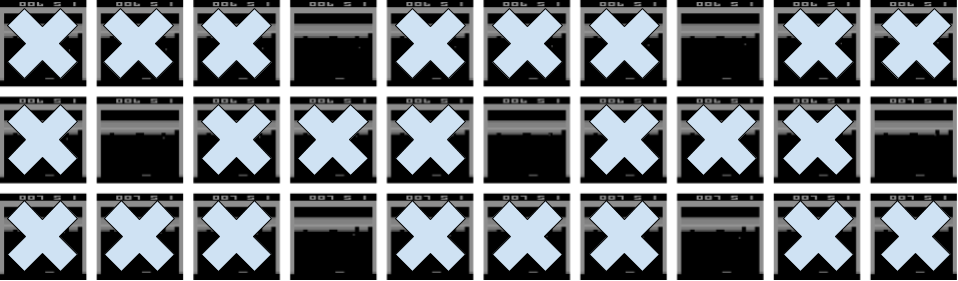
\includegraphics[width=7cm]{figures/breakout_subsampled.png}
    \end{figure}
    
    In the image there are only seven non-skipped frames: let's denote them as $x_1, x_2, \ldots, x_7$. We will use $s_1 = (x_1, x_2, x_3, x_4)$ as one state, then for the next state we will use $s_2 = (x_2, x_3, x_4, x_5)$. And so on and so forth. This is done to \alert{better discern motion}, and since the network can see up to $12$ frames ago you \alert{maximize the information} it receives.
    
    %A remark before we move on: one might be worried that the agent is throwing away a lot of information using the above procedure. In fact, it actually makes a lot of sense to do this. Seeing four consecutive frames without subsampling doesn't give enough information to discern motion that well, especially after the downsampling process.
    
\end{frame}


\begin{frame}{The Deep Q-Network}
    
    %The DQN learns an approximation of the Q-table, which is a mapping between the states and actions that an agent will take. For every state we'll have four actions that can be taken. The environment provides the state, and the action is chosen by selecting the larger of the four Q-values predicted in the output layer.
    %The policy network will return the predicted Q-values for any given state-action pairs.
    
    The DQN learns an approximation of the Q-table, which is a mapping between the states and actions that an agent will take. For every state we'll have four actions that can be taken. The environment provides the state, and the action is chosen by selecting the larger of the four Q-values for every state-action pairs predicted in the output layer.
    
    \begin{columns}[onlytextwidth]
        \begin{column}{.4\textwidth}
            \begin{itemize}[itemsep=0pt]
                \item[\alert{$\bullet$}] Input: $4 \times 84 \times 84$
                \item[\alert{$\bullet$}] Conv2d: $32 \times 20 \times 20$
                \item[\alert{$\bullet$}] Conv2d: $64 \times 9 \times 9$
                \item[\alert{$\bullet$}] Conv2d: $64 \times 7 \times 7$
                \item[\alert{$\bullet$}] Linear: $(7 \cdot 7 \cdot 64) \times 1$
                \item[\alert{$\bullet$}] Linear: $512$
                \item[\alert{$\bullet$}] Output: $4$
            \end{itemize}
        \end{column}
        
        \begin{column}{.6\textwidth}
            \begin{figure}
                \centering
                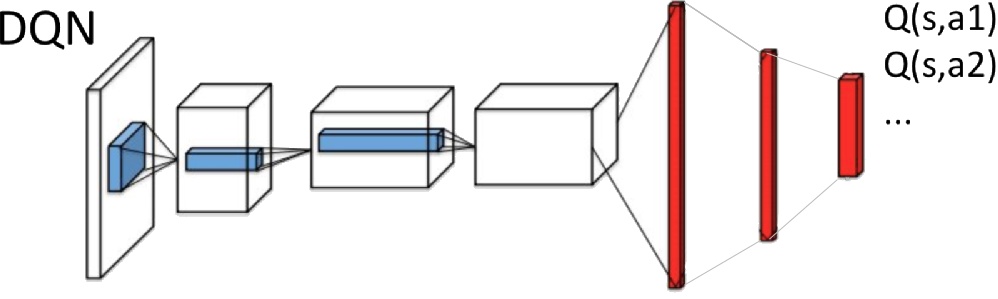
\includegraphics[width=7cm]{figures/DQN.png}
            \end{figure}
        \end{column}
    \end{columns}
    \medskip
    
    I've used a time decreasing $\varepsilon$-greedy strategy, dependent on the current time-step, to balance exploration and  exploitation.
    
\end{frame}


\begin{frame}{Double Q-Learning}

    Using only one network, when our weights update, our outputted Q-values will update, but so will our target Q-values since the targets are calculated using the same weights. So, as our Q-values move closer and closer to their targets Q-values, the targets Q-values continue to \alert{move further} and further because we're using the same network to calculate both of these values. This makes the optimization appear to be chasing its own tail, which introduces \alert{instability}. To solve this problem we will use two networks:
    
    \begin{description}
        \item[\alert{policy network}] its objective is to approximate the optimal policy by finding the optimal Q-function. It outputs an estimated Q-value for each possible action from the given input state.
        \item[\alert{target network}] its objective is to obtain the $\max$ Q-value for the next state, so to plug this value into the Bellman equation in order to calculate the target Q-value for the first state. It is a clone of the policy network: its weights are frozen with the policy network's weights, and we update them using the policy network's new weights every certain amount of time steps (an hyperparameter).
    \end{description}
    
\end{frame}


{\putbg
\section{The Journey of Learning} % The Learning Process
}


\begin{frame}{Comparison with other projects}

    Unlike Cart-pole, Breakout does not have a specified reward threshold at which it's considered solved. Some consider it to be achieving consistently $200+$ reward.
    
    The Deepmind paper trained for --- as written in \cite{Mnih2015} ---
    \begin{displayquote}
        a total of 50 million frames (that is, around 38 days of game experience in total)
    \end{displayquote}
    and it achieved a reward of $401.2 \, (\pm 26.9)$ [Extended Data Table 2].

    Looking around, on one post I've seen that it takes around $5K$ episodes or $1M$ time steps to start learning (getting a reward of around $10$).
    
    Another post trained for $5M$ steps, which took about $\sim 40$h on Tesla K80 GPU or $\sim 90$h on 2.9 GHz Intel i7 Quad-Core CPU, with a reward average of $\sim 62$.
    
    \alert{Instead}, on Ulysses I started to gain a reward of around $10$ at $40K$ episodes or $10M$ time steps.
    
    % Problems
    % The cluster and the notebooks all run out of memory. The only one that survives a bit is Google Colab, but after $5$ hours you finish the available runtime so the kernel is disconnected, and since (I really don't know why) it doesn't save the checkpoints I cannot continue the training.

\end{frame}


{\putbgdark
\begin{frame}[standout]
	\begin{center}
        %But it kept crashing.
        %It turns out, that you don't want to plot three figures every episode if you're already using a lot of memory.
        After $102$ job, for a total of $112:33:31$ hours, I got:
	\end{center}
\end{frame}
}
\stepcounter{framenumber}


\begin{frame}{The rewards are growing}

    \begin{figure}
        \centering
        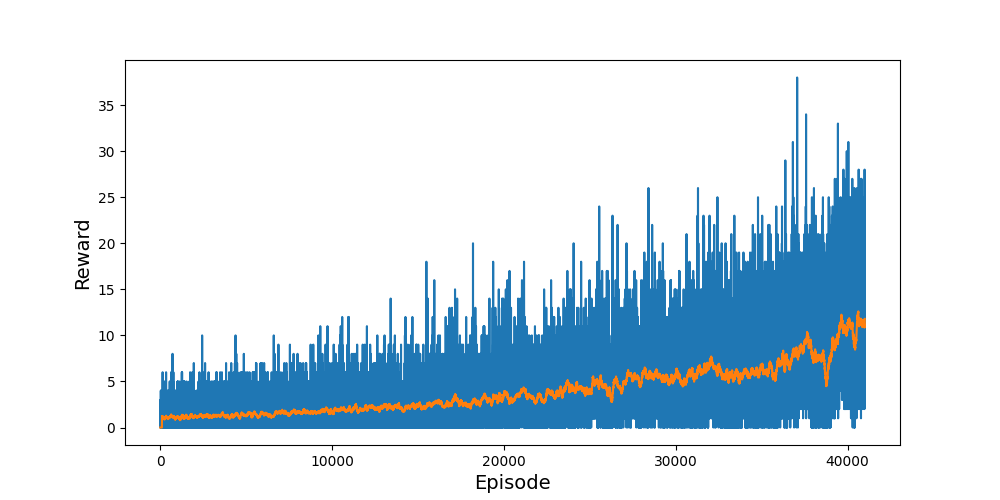
\includegraphics[width=\textwidth]{figures/rewards_02_41000.png}
    \end{figure}
    
\end{frame}


\begin{frame}{The durations are growing}

    \begin{figure}
        \centering
        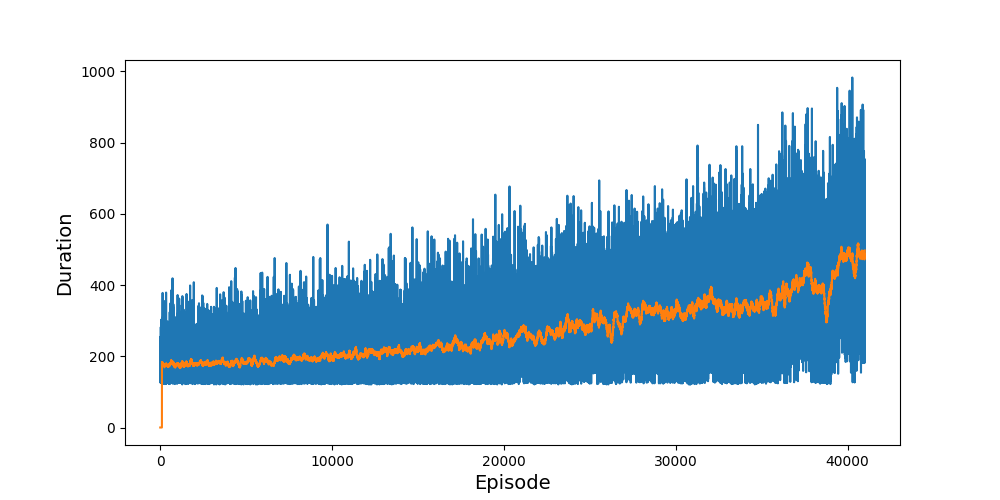
\includegraphics[width=\textwidth]{figures/durations_02_41000.png}
    \end{figure}
    
\end{frame}


\begin{frame}{The loss is decreasing (incomplete)}

    \begin{figure}
        \centering
        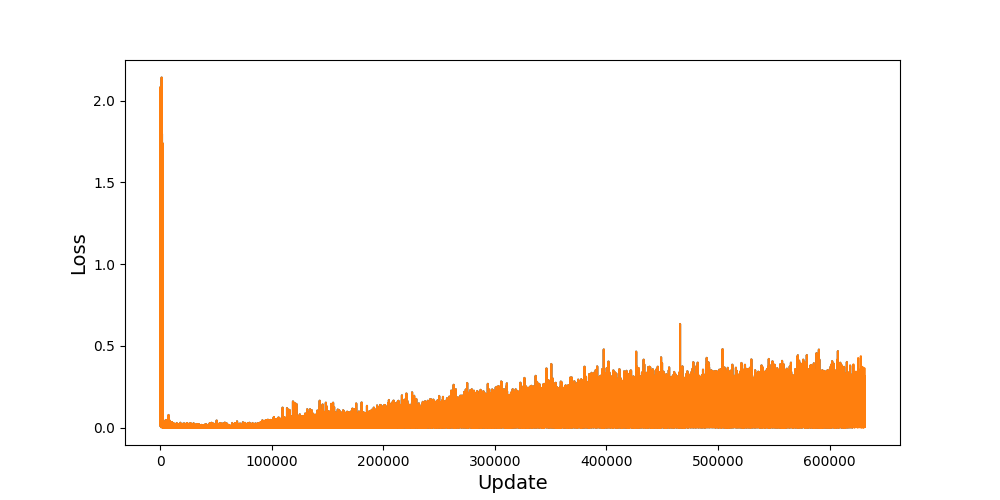
\includegraphics[width=\textwidth]{figures/loss_02_OLD.png}
    \end{figure}
    
\end{frame}


\begin{frame}{Improvements}

    What could be done better?
    \begin{itemize}
        \item[\alert{$\bullet$}] Efficient handling of the replay memory: instead of saving $4$ frames for the state and $4$ frames for the next state in each experience, use the fact that $3$ of them are equal to save some space.
        \item[\alert{$\bullet$}] Implement a dueling architecture, which splits the network into two separate streams (one for estimating the state-value $V(s)$ and the other for estimating state-dependent action advantages $A(s, a_i)$), so to generalize learning across actions (see the paper of \href{https://arxiv.org/abs/1511.06581}{Wang et al.}).
        \item[\alert{$\bullet$}] Use the environment \texttt{Breakout-ram-v0} (\href{https://gym.openai.com/envs/Breakout-ram-v0/}{documentation}), in which the observation is the content of the 128 bytes of RAM of the Atari machine. In this way the agent can learn from the individual bits.
    \end{itemize}
    
\end{frame}


{\putbgdark
\begin{frame}[standout]
	\begin{center}
		\Large \uncover<+->{Thank you for your attention!}
		
		\Huge\uncover<+->{\Smiley}
	\end{center}
\end{frame}
}


\begin{frame}[allowframebreaks, noframenumbering, plain]{}

	\nocite{*}
	\printbibliography

\end{frame}

{\putbgdark
\begin{frame}[standout]
	\begin{center}
		\Large \uncover<+->{To the game!}
		
		\Huge\uncover<+->{\faGamepad}
	\end{center}
\end{frame}
}



\end{document}